\documentclass{mcmthesis}
\mcmsetup{CTeX = false,   % 使用 CTeX 套装时,设置为 true
        tcn = 2115481, problem = A,
        sheet = true, titleinsheet = true, keywordsinsheet = true,
        titlepage = false, abstract = true}
% \usepackage[UTF8]{ctex}
\usepackage{newtxtext}%\usepackage{palatino}
\usepackage{lipsum}
\usepackage{amsmath}
\usepackage{cite}
\usepackage{url}
\usepackage{float}
\usepackage[nottoc,notlot,notlof]{tocbibind}
\title{MCM Thesis}
\begin{document}
\begin{abstract}
  Abstract here3


\begin{keywords}
keyword1; keyword2
\end{keywords}
\end{abstract}
\maketitle
%% Generate the Table of Contents, if it's needed.
\tableofcontents
\newpage
%% Generate the Memorandum, if it's needed.
% \memoto{\LaTeX{}studio}
% \memofrom{Liam Huang}
% \memosubject{Happy \TeX{}ing!}
% \memodate{\today}
% % \logo{\LARGE I'm pretending to be a LOGO!}
% \begin{memo}[Memorandum]
%   \lipsum[1-3]
% \end{memo}

\section{Introduction}
\subsection{Problem Background}

The carbon cycle process is a very vital component of the planet. Part of the carbon cycle process is the decomposition of compounds, allowing carbon to be renewed and used in other forms. A key part of the decomposition of compounds comes from the decomposition of plant material and woody fibers. Some of the key agents in decomposing woody fibers are fungi. Studies have shown that among the many fungi traits, the growth rate of the fungus and the fungus' tolerance to moisture is the growth rate of the fungus and the fungus' tolerance to moisture. There are interesting correlations between fungi traits. And when different types of fungi coexist, they will affect each other. 

\begin{figure}[H]
\small
\centering
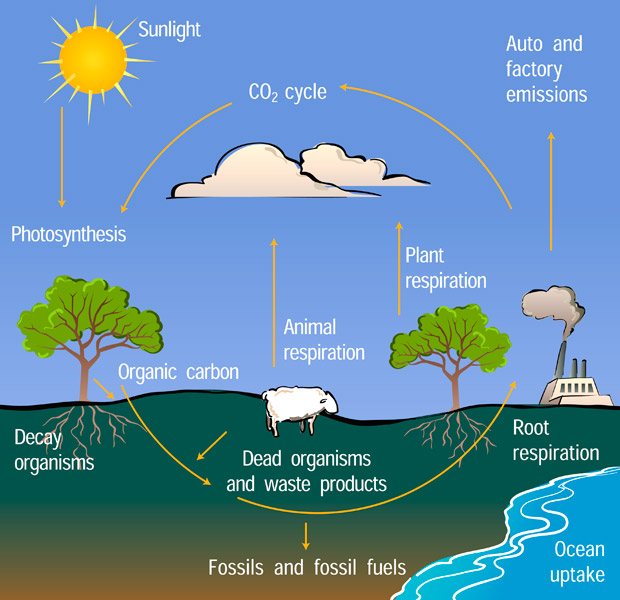
\includegraphics[width=8cm]{carbon_cycle}
\caption{A simple diagram of parts of the carbon cycle, emphasizing the terrestrial (land-based) parts of the cycle.\cite{carbon_cycle}}
\label{carbon_cycle}
\end{figure}

Thus, our team is working to better understand the relationship between traits and the competitive role of different types of fungi coexisting. In addition, it is necessary to consider the possible long-term or short-term effects of various external conditions such as different climates, seasonal changes, sudden weather, etc. 

There are many models for analyzing the relationship between various traits, such as time series, linear regression and so on. Fungi have their relatively suitable temperature, and they are sensitive to the external environment, so the model needs to be robust. For studying how the diversity of fungal communities of a system impacts the overall efficiency of a system, there are methods such as cellular automata for simulation. 

This article studies these effects, based on our proposed model, we make predictions about the relative advantages and disadvantages for each species and combinations of species likely to persist and we realize the importance and the role of biodiversity in the presence of different degrees of variability in the local environment.

\subsection{Restatement of the Problem}

Based on the relevant conclusions in the research article given in the question, our paper should continue to explore and adress the following aspects. 

\begin{itemize}
  \item \textbf{Problem 1:}
  Describe the breakdown of ground litter and woody fibers through fungal activity in the presence of multiple species of fungi.
  \item \textbf{Problem 2:}
  Incorporate the interactions between different species of fungi, which have different growth rates and different moisture tolerances.
  \item \textbf{Problem 3:}
  Describe the interactions between the different types of fungi. The dynamics of the interactions should be characterized and described including both short- and long-term trends. The sensitivity to rapid fluctuations in the environment should be examined and we have to determine the overall impact of changing atmospheric trends to assess the impact of variation of local weather patterns.
  \item \textbf{Problem 4:}
  Include predictions about the relative advantages and disadvantages for each species and combinations of species likely to persist, and do so for different environments.
  \item \textbf{Problem 5:}
  Describe how the diversity of fungal communities of a system impacts the overall efficiency of a system with respect to the breakdown of ground litter. Predict the importance and role of biodiversity in the presence of different degrees of variability in the local environment.
\end{itemize}

\subsection{Our Approach}

As the question requires us, our primary goal is to model the decomposition of woody fibers in a given patch of land, and do so in the presence of multiple types of fungi breaking down woody fibers in the same area.

We consider using a linear regression model to analyze the relationship between different traits (mainly focus on the growth rate of the fungus and the fungus' tolerance to moisture and temperature) of fungi, and their impact on the breakdown of ground litter and woody fibers. Since fungus are sensitive to external environment, and considering rapid fluctuations in the environment, we specially select a robust regression algorithm: Theil-Sen Regression. According to our evaluation, it performs much better than least squares method when outliers exist.

Since the growth rate of fungi and the tolerance to moisture need to be considered comprehensively, we integrate this in our model. The relationship between fungal decomposition rate, growth rate and moisture tolerance is obtained by using multiple linear regression algorithm. 

At the same time, we consider that usually different kinds of fungi coexist, and there is a competitive relationship between them. In the end, there may only be one kind of different kinds of fungi that will survive to the end. we describe the interactions between the different types of fungi and estabablishe a competition model, using cellular automata model to simulate the results of competition.

To predict relative advantages and disadvantages for each species and combinations of species likely to persist, we combine models above. By changing the related parameters of temperature and moisture to simulate different environmental conditions, the dual-population competition model is extended to multiple groups, and the cellular automata algorithm is used to simulate the growth of multiple groups of fungi within a certain range. Then we consider the impact of short-term and long-term climate change, and further describe the long-term trend of fungal population changes with climate. 

To describe how the diversity of fungal communities of a system impacts the overall efficiency of a system with respect to the breakdown of ground litter, we analyse biodiversity of community with Simpson index and the distriburion of species in different degrees in the same local environment.

\section{Preparation of the Models}

\subsection{Assumptions and Justifications}

By adequate analysis of the problem, to simplify our model, we make the following well-justified assumptions.

\begin{itemize}
  \item There are no natural enemies in the environment where the fungus lives. The survival of fungi is only affected by the natural environment and other fungal populations.
  \item The amount of ground litter and woody fibers is limited. When there are multiple fungal populations, there may be competition for resources.
  \item In the decomposition process of ground litter and woody fibers, the intermediate stage of decomposition is the same as other stages.
  \item Environmental conditions change within an acceptable range, and there will be no continuous and destructive extreme weather.
\end{itemize}

\subsection{Notations}

For convenience, we introduce some notations below.

\begin{table}[htb]
  \centering
  \caption{Notations}
  \begin{center}
    \begin{tabular}{cc}
      \toprule[1.5pt]
      \makebox[0.3\textwidth][c]{Symbols} & \makebox[0.4\textwidth][c]{Descriptions} \\
      \midrule[1pt]
      $M$ & Mass (mg) \\
      $t$ & Time (day) \\
      $d$ & Decomposition rate (\% mass loss over 122 days) \\
      $\rho$ & Spearman rank-order correlation coefficient \\
      $ex$ & Extension rate (mm/day) \\
      $mo$ & Moisture index ($\in [-1, 1]$) \\
      $e(n)$ & Regression error \\
      $\varepsilon_p$ & Mean square of the error \\
      $a_p(k)$ & Linear regression coefficient \\
      $D_c$ & The Simpson index of area $c$ \\
      $P_i$ & Probability of species $i$ in the sample \\
      \bottomrule[1.5pt]
    \end{tabular}
  \end{center}
\end{table}

\section{Problem 1: Single-factor Regression Model}

\subsection{Feature Selection}

In the decomposition process of ground litter and woody fibers, there are usually many kinds of fungi that work together. The quantification of the decomposition process can be described by the decomposition rate $ d $. For dead branches and leaves with a mass of $ M $, the total mass may change after the time $ t $. At any moment, its decomposition rate can be expressed as: 

\begin{equation}
  d=\frac{\delta M}{\delta t}
\end{equation}

For a given piece of land, the decomposition rate of fungi varies with the various traits of different types of fungi. In order to get the change trend of the decomposition rate and each trait first, we temporarily ignore the specific value and convert the original value into a sorted label to describe the corresponding size relationship. According to the data set, for each trait $ x $ and decomposition rate $ y $, the Spearman coefficient $ \rho $ is calculated, the algorithm is as follows: 

\begin{equation}
  \rho=\frac{\sum_{i}\left(x_{i}-\bar{x}\right)\left(y_{i}-\bar{y}\right)}{\sqrt{\sum_{i}\left(x_{i}-\bar{x}\right)^{2} \sum_{i}\left(y_{i}-\bar{y}\right)^{2}}}
\end{equation}

We sort the calculation results corresponding to each trait according to the Spearman coefficient. 

\begin{figure}[H]
  \small
  \centering
  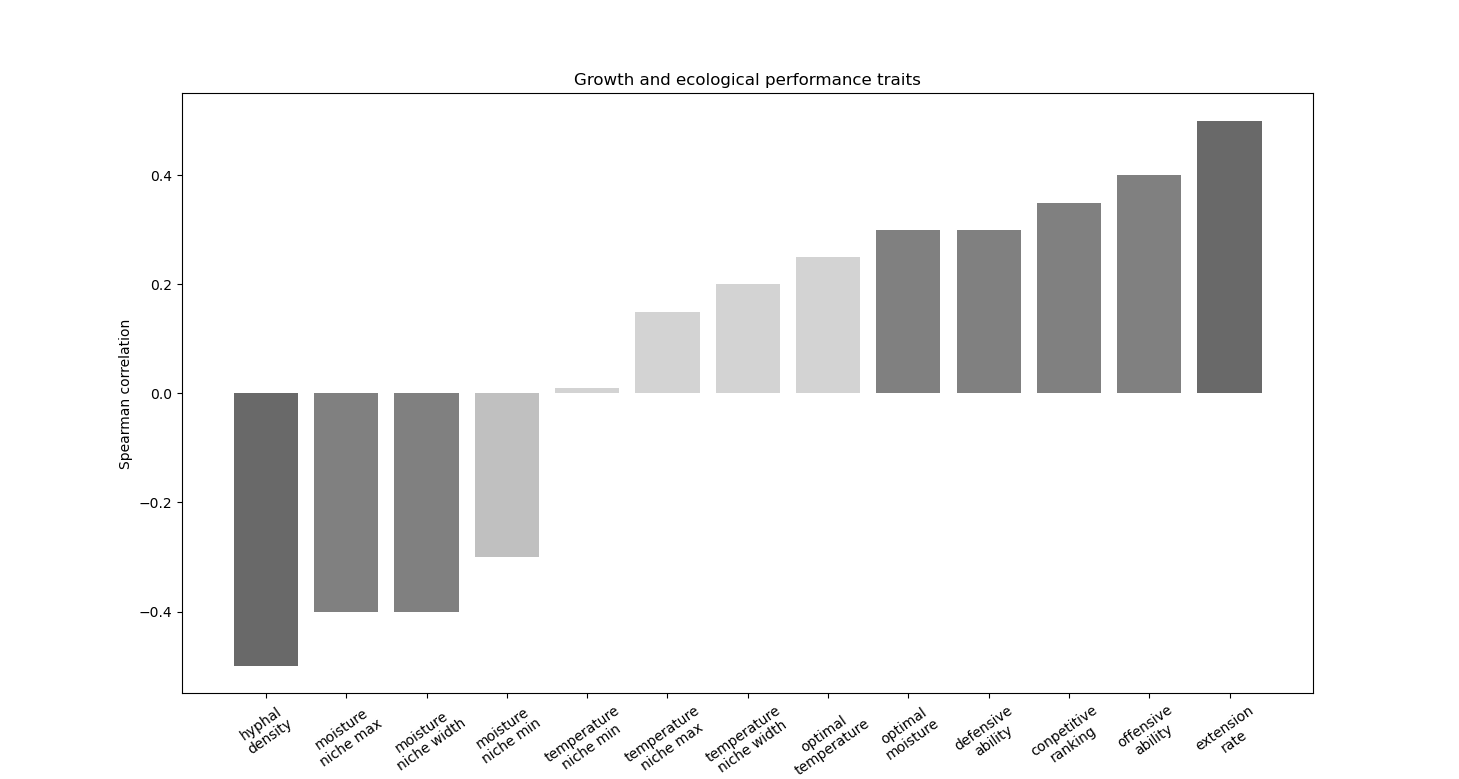
\includegraphics[width=12cm]{growth_eco_traits}
  \caption{The spearman correlation of different growth and ecological preformance traits.}
  \label{growth_eco_traits}
\end{figure}

The results show that the growth rate and moisture tolerance of fungi are closely related to the decomposition process. 

Below, based on the decomposition data of 34 species of single fungus populations collected under the condition of coexistence of multiple fungi, we will regression and predict the decomposition rate of fungi, focusing on the growth rate of a single type of hyphae The relationship with decomposition rate, and the relationship between hyphae's moisture resistance and decomposition rate. 

\subsection{The Fundamentals of Linear Regression}

The basic concept of linear regression model is that the sum of squares of the difference between the actual sampling and the linear prediction sampling reaches the minimum value, that is , the approximation of the minimum mean square error can determine the unique set of predictor coefficients.\cite{cao2009linear}

In the process of model parameter estimation, the following systems is called linear predictor.

\begin{equation}
  \hat{x}(n)=\sum_{k=1}^{p} \omega_{p}(k) x(n-k)
\end{equation}

Let $\omega_{p}(k)$ be the linear predictive coefficient and $p$ is the predictive order. The prediction error function is

\begin{equation}
  e(n)=x(n)-\hat{x}(n)
\end{equation}

That is

\begin{equation}
  e(n)=x(n)-\sum_{k=1}^{p} \omega_{p}(k) x(n-k)
  \label{alg_a}
\end{equation}

Let

\begin{equation}
  a_{p}(k)=-\omega_{p}(k)
\end{equation}

Then, (\ref{alg_a}) becomes

\begin{equation}
  e(n)=x(n)+\sum_{k=1}^{p} \omega_{p}(k) x(n-k)
  \label{alg_b}
\end{equation}

The mean square of the error is $\varepsilon_{p}=\sum_{n=p}^{N}|e(n)|^{2}$. To minimize the mean square value of the error, that is, the partial derivative is zero.

\begin{equation}
  \frac{\partial \varepsilon_{p}}{\partial a_{p}(k)}=\frac{\partial \sum_{n=p}^{N}|e(n)|^{2}}{\partial a_{p}(k)}=2 \sum_{n=p}^{N}[e(n) x(n-k)]=0
  \label{alg_c}
\end{equation}

That is

\begin{equation}
  \frac{\partial \varepsilon_{p}}{\partial a_{p}(k)}=2 \sum_{n=p}^{N}[e(n) x(n-k)]=0
\end{equation}

Substituting (\ref{alg_b}) into (\ref{alg_c}), we get

\begin{equation}
  \sum_{n=p}^{N}\left\{\left[x(n)+\sum_{k=1}^{p} a_{p}(k) x(n-k)\right] x(n-k)\right\}=\sum_{n=p}^{N} x(n) \cdot x(n-k)+\sum_{k=1}^{p} a_{p}(k) \cdot \sum_{n=p}^{N}[x(n-k) \cdot x(n-k)]
  \label{alg_d}
\end{equation}

Let

\begin{equation}
  \sum_{n=p}^{N} x(n) \cdot x(n-k)+\sum_{k=1}^{p} a_{p}(k) \cdot \sum_{n=p}^{N}[x(n-k) \cdot x(n-k)]=0
\end{equation}

In the finite sampling interval, the autocorrelation function of the real field is defined as

\begin{equation}
  r_{x}(k)=\sum_{n=k}^{N} x(n) \cdot x(n-k)(k=0,1, \cdots, p)
  \label{alg_e}
\end{equation}

Substituting (\ref{alg_e}) into (\ref{alg_d}), we get

\begin{equation}
  r_{x}(k)+\sum_{k=1}^{p} a_{p}(k) r_{x}(n-k)=0
\end{equation}

That is

\begin{equation}
  \sum_{k=1}^{p} a_{p}(k) r_{x}(n-k)=-r_{x}(k)
  \label{alg_f}
\end{equation}

We represent (\ref{alg_f}) as a matrix.

\begin{equation}
  \left(\begin{array}{cccc}
  r_{x}(0) & r_{x}(1) & \cdots & r_{x}(p-1) \\
  r_{x}(1) & r_{x}(0) & \cdots & r_{x}(p-2) \\
  \vdots & \vdots & \ddots & \cdots \\
  r_{x}(p-1) & r_{x}(p-2) & \cdots & r_{x}(0)
  \end{array}\right)\left(\begin{array}{c}
  a_{p}(1) \\
  a_{p}(2) \\
  \vdots \\
  a_{p}(p)
  \end{array}\right)=-\left(\begin{array}{c}
  r_{x}(1) \\
  r_{x}(2) \\
  \vdots \\
  r_{x}(p)
  \end{array}\right)
\end{equation}

\subsection{Decomposition Rate and Moisture Relationship}

We normalize the size of the optimal moisture range of fungus as the abscissa, $ \text {mo}=\frac{2 \times \text {width }}{\text {maxwidth }}-1 $. The zero point is the center, -1 means the fungus has the strongest moisture adaptability, and 1 means the fungus has the narrowest suitable moisture range. Plotting a scatter plot shows that the moisture resistance and decomposition rate are negatively correlated. Combining the decomposition rate of various fungi with different moisture adaptability under the same experimental conditions, using one-variable linear regression, the linear equation obtained is 

\begin{equation}
  \log {d}=1.00mo+1.74,R^2=0.3981
\end{equation}

That is

\begin{equation}
  {d}=10 ^{1.00mo+1.74}
\end{equation}

It indicates that the greater the $mo $, the worse the adaptability of the fungus and the greater the decomposition rate. It also shows that the ability of fungi to adapt to moisture is negatively related to the decomposition rate. 

\begin{figure}[H]
  \small
  \centering
  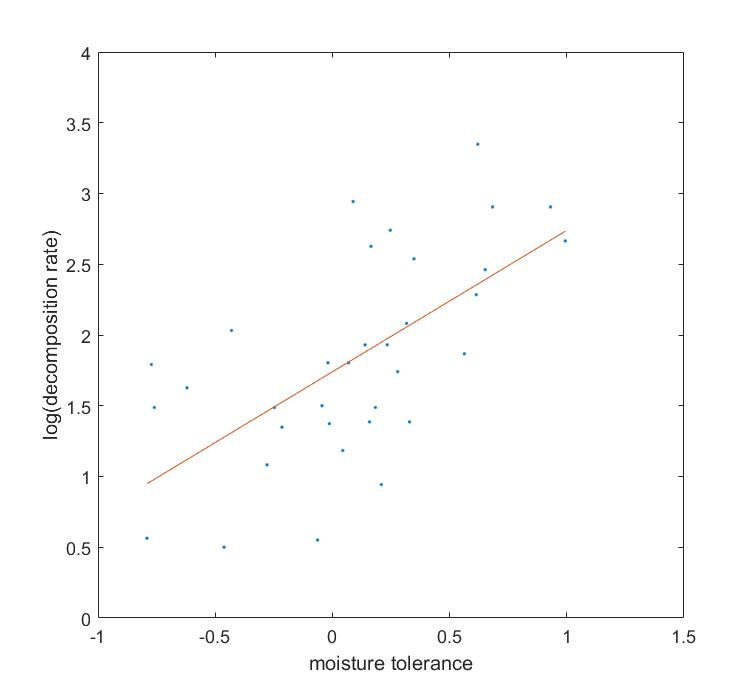
\includegraphics[width=8cm]{decomposition_moisture}
  \caption{The relationship between the moisture tolerance of various fungi and the resulting wood decomposition rate.}
  \label{decomposition_moisture}
\end{figure}

\subsection{Decomposition Rate and Extension Rate Relationship}

Then we control the moisture to remain unchanged. Taking into account the influence of temperature on the decomposition rate,  We perform linear fitting on the depositoin rate and the hypohal extension rate under $ T=10, 16, 22^{\circ}C $ respectively. We get the following results. 

\begin{figure}[H]
  \small
  \centering
  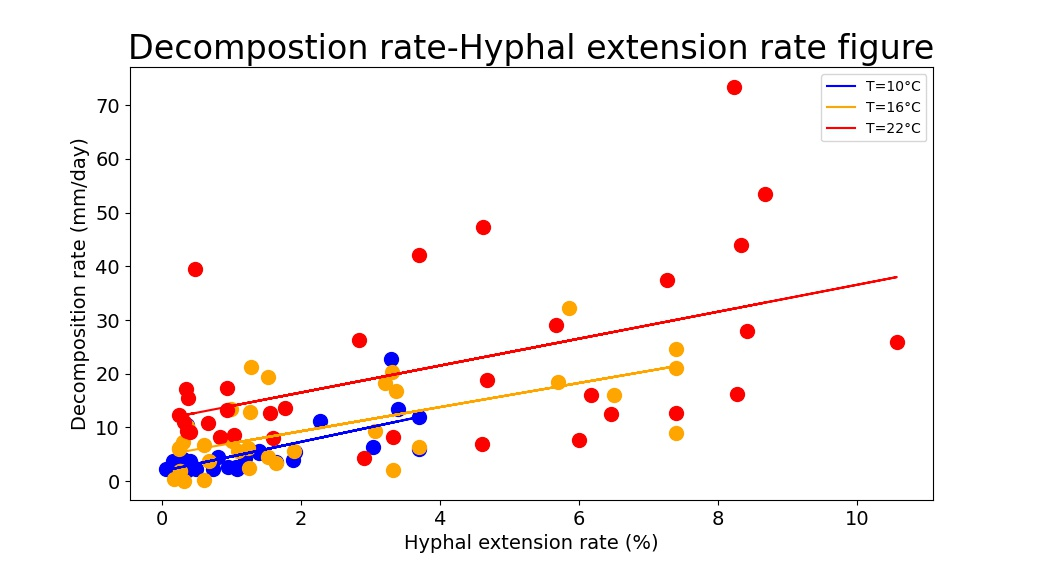
\includegraphics[width=12cm]{decomposition-extension_tot}
  \caption{The relationship between the hyphal extension rate (mm/day) of various fungi and the resulting wood decomposition rate (\% mass loss over 122 days) at various temperatures. \cite{lustenhouwer2020trait} According to the data given in the article's appendix, we re-mapped.}
  \label{decomposition-extension_tot}
\end{figure}

The corresponding equations and their correlation coefficients are: 

\begin{equation}
  \begin{split}
    d&=2.73ex+1.86,R^2=0.5009 (T=10^{\circ}C) \\
    d&=2.25ex+4.80,R^2=0.4147 (T=16^{\circ}C) \\
    d&=2.51ex+11.48,R^2=0.2511 (T=22^{\circ}C)
  \end{split}
\end{equation}

The correlation coefficient $ R^{2} $ of the linear regression model is not high. And as the temperature rises, $ R^{2} $ decreases, indicating that in a warmer soil environment, the actual relationship is more complicated than linear association. However, the model has sufficiently reflected that the decomposition rate is negatively correlated with moisture resistance. And there is a positive correlation with its extension rate.

\section{Multi-factor Regression Model}

\subsection{Problem Analysis}

In different climates, the decomposition rate of fungi is different. Even in areas with the same climate, with the changes in soil temperature, moisture and other factors, there are big differences between different parts of the fungus selected. This difference is caused by the mutual influence and interaction of many factors. Relying solely on the control variables to study the influence of certain factors on the decomposition rate is not enough to reflect the actual situation. 

According to the conclusion in question 1, the decomposition rate of ground litter and woody fibers by fungi is mainly related to the growth rate and moisture resistance of fungi. In order to comprehensively consider the influence of the two factors, we need to merge the two relationships in question 1. 

We assume that fungal growth rate and moisture tolerance are two intrinsic traits that are independent of each other. On the basis of the unary linear model in question 1, we build a multiple linear regression model. 

\subsection{Incorporate the Interactions}

Consider the situation at $16 ^ \circ C $. First, control the decomposition rate $ y $ in Model 1 unchanged. We calculate the corresponding extension rate $ x_0 $ and moisture tolerance $ x_1 $ at this time. Take some points $ (y,x_0,x_1) $ as shown in the following table: 

\begin{table}[htb]
  \centering
  \caption{Decomposition rate and extension rate and moisture relationship}
  \begin{center}
    \begin{tabular}{ccccccc}
      \toprule[1.5pt]
      \makebox[0.1\textwidth][c]{Parameter} & \makebox[0.1\textwidth][c]{Point 1} & \makebox[0.1\textwidth][c]{Point 2} & \makebox[0.1\textwidth][c]{Point 3} & \makebox[0.1\textwidth][c]{Point 4} & \makebox[0.1\textwidth][c]{Point 5} & \makebox[0.1\textwidth][c]{Point 6}\\
      \midrule[1pt]
      $y$ & 5 & 10 & 20 & 30 & 40 & 50 \\
      $x_0$ & -1.04 & -0.74 & -0.44 & -0.26 & -0.14 & -0.04 \\
      $x_1$ & 0.09 & 2.31 & 3.20 & 3.64 & 4.09 & 20.09 \\
      \bottomrule[1.5pt]
    \end{tabular}
  \end{center}
\end{table}

We assume that the decomposition rate $ Y $, the growth rate $ x_0 $ and the humidity resistance $ x_1 $ satisfy the following linear relationship: 

\begin{equation}
  Y(x)=h_\theta(x)=\theta^{\top} x=\theta_{0} x_{0}+\theta_{1} x_{1}
\end{equation}

Where

\begin{equation}
  \boldsymbol{Y}=\left(\begin{array}{c}
  y_{1} \\
  y_{2} \\
  \vdots \\
  y_{n}
  \end{array}\right), \boldsymbol{X}=\left(\begin{array}{cccc}
  1 & x_{11} & \cdots & x_{1 p} \\
  1 & x_{21} & \cdots & a_{2 p} \\
  \vdots & \vdots & \ddots & \vdots \\
  1 & x_{n 1} & \cdots & a_{n p}
  \end{array}\right), \boldsymbol{\theta}=\left(\begin{array}{c}
  \theta_{0} \\
  \theta_{1} \\
  \vdots \\
  \theta_{p}
  \end{array}\right), \boldsymbol{\varepsilon}=\left(\begin{array}{c}
  \varepsilon_{1} \\
  \varepsilon_{2} \\
  \vdots \\
  \varepsilon_{n}
  \end{array}\right)
\end{equation}

Introduce a cost function to measure the regression effect:

\begin{equation}
  J\left(\theta_{0}, \theta_{1}\right)=\frac{1}{2 m} \sum_{i=1}^{m}\left(h_{\theta}\left(x^{(i)}\right)-y^{(i)}\right)^{2}
\end{equation}

To apply the gradient descent method to our previous linear regression problem, the key is to find the derivative of the cost function, namely: 

\begin{equation}
  \frac{\partial}{\partial \theta_{j}} J\left(\theta_{0}, \theta_{1}\right)=\frac{\partial}{\partial \theta_{j}} \frac{1}{2 m} \sum_{i=1}^{m}\left(h_{\theta}\left(x^{(i)}\right)-y^{(i)}\right)
\end{equation}

When $ j=0 $:

\begin{equation}
  \frac{\partial}{\partial \theta_{0}} J\left(\theta_{0}, \theta_{1}\right)=\frac{1}{m} \sum_{i=1}^{m}\left(h_{\theta}\left(x^{(i)}\right)-y^{(i)}\right)
\end{equation}

When $ j=1 $:

\begin{equation}
  \quad \frac{\partial}{\partial \theta_{1}} J\left(\theta_{0}, \theta_{1}\right)=\frac{1}{m} \sum_{i=1}^{m}\left(\left(h_{\theta}\left(x^{(i)}\right)-y^{(i)}\right) \cdot x^{(i)}\right)
\end{equation}

Then iterate the following formulas

\begin{equation}
  \begin{split}
    \begin{array}{l}
      \theta_{0}:=\theta_{0}-a \frac{1}{m} \sum_{i=1}^{m}\left(h_{\theta}\left(x^{(i)}\right)-y^{(i)}\right) \\
      \theta_{1}:=\theta_{1}-a \frac{1}{m} \sum_{i=1}^{m}\left(\left(h_{\theta}\left(x^{(i)}\right)-y^{(i)}\right) \cdot x^{(i)}\right)
    \end{array}
  \end{split}
\end{equation}

Substitute each group of observations in the above table to estimate the regression coefficient by least squares. Regression solving the above algorithm, the regression equation is $ Y = 35.129x_0 +0.667x_1 + 37.692 $. That is $ d = 35.129ex +0.667mo + 37.692 $ 

The regression plane in the three-dimensional space is shown in the figure below.

\begin{figure}[H]
  \small
  \centering
  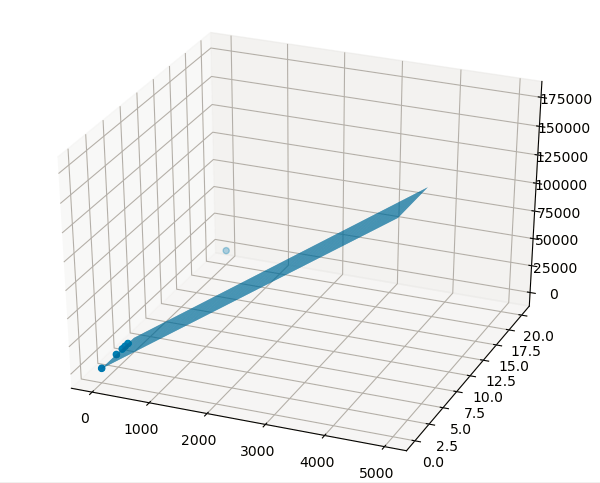
\includegraphics[width=10cm]{3dim_de_extension_moi}
  \caption{Relationship between fungi decomposition rate and growth rate and moisture tolerance.}
  \label{3dim_de_extension_moi}
\end{figure}

The result is $ \theta_0\ne0,\theta_1\ne 0 $, indicating that the regression model is effective.






















































\bibliography{ref}{}
\bibliographystyle{plain}

\begin{appendices}

\section{Article}

In addition, 

\begin{letter}{Dear, Mr. Alpha Chiang}

its a letter

\vspace{\parskip}

Sincerely yours,

Your friends

\end{letter}
Here are simulation programmes we used in our model as follow.\\


\section{Programs}
\textbf{\textcolor[rgb]{0.98,0.00,0.00}{Input Python source:}}
\lstinputlisting[language=Python]{./code/extension_decomposition_temp.py}
\end{appendices}
\end{document}